\ProvidesFile{section_6_jordan}[Section 6]

\newpage

\section{Triangular and Jordan Normal Forms}

\begin{center}
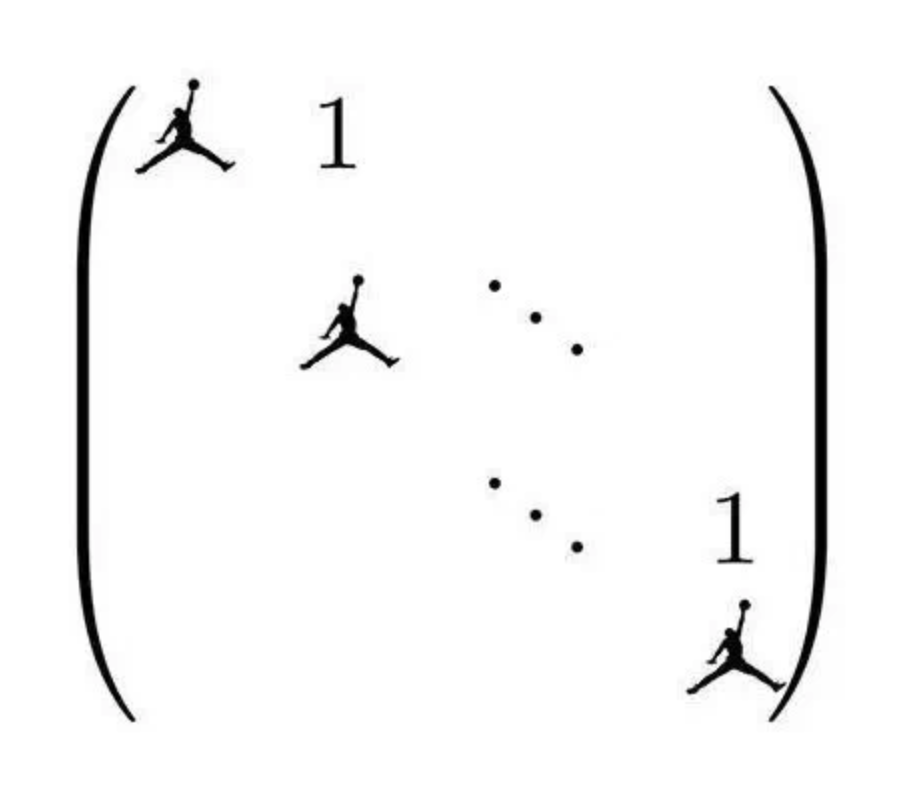
\includegraphics[scale=0.12]{Images/jordan.png}
\end{center}

In this section, we consider linear operators when a basis of eigenvectors is not available.

As usual, we consider a linear operator $\A\colon V \to V$, where $V$ is a vector space over $\F$ and $\dim V = n$. In this section, we work over $\C$ (or over $\R$ when the characteristic polynomial has $n$ real roots counted with multiplicity).

\subsection{Invariant subspaces}

\begin{definition}
The eigenspace of a linear operator $\A\colon V \to V$ corresponding to an eigenvalue $\lambda$ is the set of vectors $V_{\lambda}(\A) = \{v \in V \mid \A(v) = \lambda v\} = \nul(\A - \lambda I)$.
\end{definition}

\begin{exercise}
The eigenspace is a subspace of $V$.
\end{exercise}

\begin{remark}
The set of all eigenvectors corresponding to a given eigenvalue $\lambda$ is $V_{\lambda}(\A)\setminus\{0\}$.
\end{remark}

\begin{definition}
    A subspace $W$ of $V$ is called invariant under a linear operator $\A\colon V \to V$ if $\A(W) \subseteq W$.
\end{definition}
    
\begin{exercise}
    If a linear operator has an eigenvector, then the subspace spanned by that eigenvector is invariant under the linear operator.
\end{exercise}
    
\begin{exercise}
        If a linear operator has an eigenspace, then that eigenspace is invariant under the linear operator.
\end{exercise}
    
\begin{exercise}
    If a subspace $W$ is invariant under a linear operator $\A\colon V \to V$, then the restriction of $\A$ to $W$ is a linear operator on $W$.
\end{exercise}

\begin{exercise}
    What is the form of the matrix of a linear operator in a basis adapted to an invariant subspace? (The invariant subspace's basis is a part of the basis of the whole space.)
\end{exercise}

\begin{exercise}
    What happens to the matrix if the space is represented as a direct sum of invariant subspaces?
\end{exercise}

\begin{definition}
The algebraic multiplicity of an eigenvalue $\lambda$ is the multiplicity of $\lambda$ as a root of the characteristic polynomial.
\end{definition}

\begin{definition}
The geometric multiplicity of an eigenvalue $\lambda$ is the dimension of the eigenspace $V_{\lambda}(\A)$.
\end{definition}

\begin{lemma}
The algebraic multiplicity of an eigenvalue $\lambda$ is greater than or equal to its geometric multiplicity.
\end{lemma}

\begin{proof}
The eigenspace $V_{\lambda}(\A)$ is an invariant subspace of $\A$. Extend it to a basis of the whole space and write the matrix of $\A$ in this basis:
$$
A = \begin{pmatrix}
\lambda I_k & * \\
0 & B \\
\end{pmatrix},
$$
where $k = \dim V_{\lambda}(\A)$.

Then the characteristic polynomial of $\A$ equals $(t - \lambda)^k \det(t I_{n - k} - B)$. Hence, the algebraic multiplicity of the eigenvalue $\lambda$ is greater than or equal to $k = \dim V_{\lambda}(\A)$.
\end{proof}

\begin{lemma}
The sum of the eigenspaces of a linear operator corresponding to different eigenvalues is direct.
\end{lemma}

\begin{exercise}
Prove the lemma.
\end{exercise}

Then the following theorem holds:

\begin{theorem}
A linear operator is diagonalizable if and only if the algebraic multiplicity of each eigenvalue is equal to its geometric multiplicity.
\end{theorem}

\begin{exercise}
Prove the theorem.
\end{exercise}

We will now spend some time understanding what to do when an operator is not diagonalizable.

\subsection{Triangular Form}

First, we show that any complex linear operator can be brought to an upper-triangular form in some basis.

From the previous section, we know that every complex linear operator has at least one one-dimensional invariant subspace (spanned by an eigenvector).

\begin{lemma}
Any complex linear operator has an $(n-1)$-dimensional invariant subspace.
\end{lemma}

\begin{proof}
Consider the linear operator $\A^{*}\colon V^{*} \to V^{*}$ over $\C$ with $\dim V = \dim V^{*} = n$. Then $\A^{*}$ has an eigenvector $f \in V^{*}$ with eigenvalue $\lambda \in \C$. Since $f$ is a nonzero linear functional (a single row in coordinates), its kernel (the solution set of the homogeneous linear equation $f(v) = 0$) has dimension $n-1$.

Let us prove that $\ker f$ is invariant under $\A$. Assume $v \in \ker f$. Then $0 = f(v) = \lambda f(v) = (\lambda f)(v) = (\A^{*}f)(v) = f(\A v)$, hence $\A v \in \ker f$. Thus, $\ker f$ is an $(n-1)$-dimensional invariant subspace of $\A$.
\end{proof}

\begin{corollary}\label{triangular_form}
Any complex linear operator has an upper-triangular matrix in some basis.
\end{corollary}

\begin{exercise}
Prove the corollary by induction on the dimension of the space.
\end{exercise}

\subsection{Annihilating polynomials}

We now work with polynomials in matrices and operators. For a polynomial $p(x) = a_m x^m + \cdots + a_1 x + a_0$, define the polynomial in a matrix $A$ as $p(A) = a_m A^m + \cdots + a_1 A + a_0 I$ ($I$ is the identity matrix of the same size as $A$) and the polynomial in an operator $\A$ as $p(\A) = a_m \A^m + \cdots + a_1 \A + a_0 I$ ($I$ is the identity on $V$).

\begin{exercise}
Prove that $p(\A)$ is a linear operator on $V$.
\end{exercise}

\begin{exercise}
Let $p(x) = x^2 - 3x + 1$. Compute $p(A)$ for
$$A = \begin{pmatrix} 1 & 0 & 0 \\ 0 & -1 & 0 \\ 0 & 0 & 2 \end{pmatrix}.$$
\end{exercise}

\begin{exercise}
Show that for any polynomials $p(x)$ and $q(x)$, we have $p(A)q(A) = q(A)p(A)$ (even though two arbitrary matrices or operators do not commute).
\end{exercise}

\begin{definition}
An annihilating polynomial of a linear operator $\A$ is a polynomial $p(x)$ such that $p(\A) = 0$ (the zero operator on the right-hand side).
\end{definition}

\begin{exercise}
    Prove that $x^2 - 1$ is an annihilating polynomial of the matrix 
    $$A = \begin{pmatrix} 1 & -4 \\ 0 & -1 \end{pmatrix}.$$
\end{exercise}

\begin{exercise}
    Prove that $x^3$ is an annihilating polynomial of the matrix 
    $$A = \begin{pmatrix} 0 & 2 & 2 \\ 0 & 0 & 2 \\ 0 & 0 & 0 \end{pmatrix}.$$
\end{exercise}
(Recall the definition of a nilpotent matrix from the previous section.)

\begin{exercise}
Find an annihilating polynomial for a projection (idempotent) matrix.
\end{exercise}

\begin{definition}
Minimal polynomial of a linear operator $\A$ is a monic polynomial $m(x)$ of the smallest degree such that $m(\A) = 0$.
\end{definition}

\begin{theorem}
The minimal polynomial of a linear operator exists and is unique. Moreover, the degree of the minimal polynomial is less than or equal to $n^2$. (We will be able to even decrease it to $n$ later.)
\end{theorem}

\begin{proof}
Consider elements 
$$
I, A, A^2, \ldots, A^{n^2}
$$
in the $n^2$-dimensional vector space $M_n(\F)$. Since there are $n^2 + 1$ elements, they are linearly dependent. Hence, there exist scalars $c_0, c_1, \ldots, c_{n^2}$, not all zero, such that 
$$
c_0 I + c_1 A + c_2 A^2 + \ldots + c_{n^2} A^{n^2} = 0.
$$
Hence, $m(x) = c_0 + c_1 x + c_2 x^2 + \ldots + c_{n^2} x^{n^2}$ is an annihilating polynomial of $\A$.

Then we can choose an annihilating polynomial of the smallest degree. Dividing by the leading coefficient, we get a monic polynomial.

Now assume that there are two minimal polynomials $m(x)$ and $m'(x)$ of the same degree. Then $m(x) - m'(x)$ is an annihilating polynomial of degree less than the degree of $m(x)$ and $m'(x)$. Hence, $m(x) = m'(x)$.
\end{proof}

\begin{theorem}
Any annihilating polynomial of a linear operator $\A$ is divisible by the minimal polynomial of the operator.
\end{theorem}

\begin{exercise}
Prove the theorem using the division algorithm for polynomials.
\end{exercise}

\begin{exercise}
Find the minimal polynomial of a projection, a nilpotent operator, and a rotation of the real plane by $2\pi/3$.
\end{exercise}

\begin{theorem}[Cayley-Hamilton theorem]
The characteristic polynomial of a linear operator (and its matrix) is an annihilating polynomial of the operator (and the matrix).
\end{theorem}

\begin{proof}
Since this statement does not depend on the choice of basis, it is natural to apply Corollary~\ref{triangular_form} and assume that the matrix $A$ in some basis $(e_1, \ldots, e_n)$ is upper triangular. Consider the chain of $\mathcal{A}$-invariant subspaces

    $$
    V=V_0 \supset V_1 \supset \ldots \supset V_{n-1} \supset V_n=0
    $$
    
    where $V_k=\left\langle e_1, e_2, \ldots, e_{n-k}\right\rangle$. Since $\left(\mathcal{A}-\lambda_{n-k} I\right) e_{n-k} \in V_{k+1}$, it follows that
    $$
    \left(\A-\lambda_{n-k} I\right) V_k \subset V_{k+1}.
    $$
    Therefore,
    
    $$
    \begin{aligned}
    & \chi_{\mathcal{A}}(\mathcal{A}) V=\prod_{i=1}^n\left(\mathcal{A}-\lambda_i I\right) V= \\
    & =\left(\mathcal{A}-\lambda_1 I\right) \ldots\left(\mathcal{A}-\lambda_n I\right) V_0 \subset\left(\mathcal{A}-\lambda_1 I\right) \ldots\left(\mathcal{A}-\lambda_{n-1} I\right) V_1 \subset \\
    & \quad \subset\left(\mathcal{A}-\lambda_1 I\right) \ldots\left(\mathcal{A}-\lambda_{n-2} I\right) V_2 \subset \ldots \subset\left(\mathcal{A}-\lambda_1 I\right) V_{n-1}=0
    \end{aligned}
    $$
    
    
    Consequently, $\chi_{\A}(\A) V=0$, that is, $\chi_{\A}(\A)=0$.
\end{proof}

\subsection{Generalized eigenspaces}

\begin{definition}
\underline{\it Generalized eigenspace} of a linear operator $\A\colon V \to V$ corresponding to an eigenvalue $\lambda$ is the set of vectors $V^{\lambda} = \{v \in V \mid (\A - \lambda I)^k v = 0 \text{ for some } k \geqslant 0\}$.
\end{definition}

\begin{exercise}
Prove that the generalized eigenspace is a subspace of $V$ that is invariant under $\A$.
\end{exercise}

\begin{definition}
\underline{\it Generalized eigenvector of rank} $m$ corresponding to the eigenvalue $\lambda$ is a vector $v$ such that $(\A - \lambda I)^m v = 0$ and $(\A - \lambda I)^{m - 1} v \neq 0$.
\end{definition}

The unique generalized eigenvector of rank 0 is the zero vector; generalized eigenvectors of rank 1 are the ordinary eigenvectors.

Consider the following sequence of subspaces:
$$
\{0\} \subset \nul(\A - \lambda I) \subset \nul(\A - \lambda I)^2 \subset \ldots \subset \nul(\A - \lambda I)^m \subset \ldots.
$$

It cannot be strictly increasing infinitely, because the dimension of the space is finite. Moreover, if for the first time at some $m$ we have $\nul(\A - \lambda I)^m = \nul(\A - \lambda I)^{m + 1}$, then the chain stabilizes: all later subspaces $\nul(\A - \lambda I)^k$ ($k > m$) are equal to $\nul(\A - \lambda I)^m$. In this case $m \leqslant \dim V$. Hence, $V^{\lambda} = \{v \in V \mid (\A - \lambda I)^n v = 0\}$, where $n = \dim V$.

We have seen earlier that for some operators we cannot find a basis of eigenvectors (even over $\C$). However, we can find a basis of generalized eigenvectors. Our next goal is to prove that for any linear operator on a finite-dimensional complex vector space $V$, the space $V$ can be represented as a direct sum of generalized eigenspaces corresponding to different eigenvalues.

\begin{theorem}
Let $\mathcal{A}: V \rightarrow V$ be a linear operator, $\dim V = n$. And let its characteristic polynomial have $n$ roots counting multiplicities:

    $$
    \chi_{\mathcal{A}}(t)=\prod_{i=1}^p\left(t-\lambda_i\right)^{n_i} ; \quad \lambda_i \neq \lambda_j \text{ for } i \neq j
    $$
    (always true over $\C$).
    
Then 
\begin{enumerate}[(1)]
    \item $V=V^{\lambda_1} \oplus \ldots \oplus V^{\lambda_p}$ is a direct sum of generalized eigenspaces corresponding to distinct eigenvalues;
    \item each generalized eigenspace is invariant under $\A$;
    \item $\dim V^{\lambda_i} = n_i$ (the algebraic multiplicity of $\lambda_i$) for each $i = 1, \ldots, p$;
    \item the operator $\A - \lambda_i I$ is nilpotent on $V^{\lambda_i}$;
    \item the operator $\A - \lambda_i I$ is injective on $$
V_i=V\left(\lambda_1\right) \oplus \ldots \oplus V\left(\lambda_{i-1}\right) \oplus V\left(\lambda_{i+1}\right) \oplus \ldots \oplus V\left(\lambda_p\right);
$$
\item $\lambda_i$ is the only eigenvalue of the operator $\left.\mathcal{A}\right|_{V^{\lambda_i}}$.
\end{enumerate}
\end{theorem}

\begin{proof}
Introduce notation:
$$
\chi_i(t)=\prod_{j \neq i}\left(t-\lambda_j\right)^{n_j}, \quad i=1,2, \ldots, p.
$$
Since $\left(\chi_1(t), \ldots, \chi_p(t)\right)=1$, there exist polynomials $f_1(t), \ldots, f_p(t)$ such that 
$$
\sum_{i=1}^p \chi_i(t) f_i(t)=1.
$$
Also define the subspaces
$$
W_i=\chi_i(\mathcal{A}) f_i(\mathcal{A}) V=\left\{\chi_i(\mathcal{A}) f_i(\mathcal{A}) v \mid v \in V\right\}, \quad 1 \leqslant i \leqslant p.
$$

The subspaces $W_i$ 
\begin{itemize}
\item are invariant under $\mathcal{A}$:
$$
\mathcal{A} W_i= \mathcal{A}~\chi_i(\mathcal{A}) f_i(\mathcal{A}) V=\chi_i(\mathcal{A}) f_i(\mathcal{A}) \mathcal{A} V \subset \chi_i(\mathcal{A}) f_i(\mathcal{A}) V=W_i;
$$
\item are contained in the corresponding subspaces $V^{\lambda_i}$ (in fact, they coincide; we will see this later):
$$
\left(\A-\lambda_i I\right)^{n_i} W_i=\chi_{\A}(\A) f_i(\A) V=\text{[by the Cayley--Hamilton theorem, } \chi_{\A}(\A) =  0 \text{]}=0, 
$$
hence $W_i \subset V^{\lambda_i};$
\item their sum equals the whole space $V$:
substitute the operator $\mathcal{A}$ into the identity decomposition and obtain 
$$\sum_{i=1}^p \chi_i(\A) f_i(\A)=I,$$
then any vector $v \in V$ can be written as 
$$v = \sum_{i=1}^p \chi_i(\A) f_i(\A) v \in \sum_{i=1}^p W_i, \text{ hence } V = \sum_{i=1}^p W_i. $$
\end{itemize}

Therefore, from $W_i\subset V^{\lambda_i}$ we get $$V =  \sum_{i=1}^p V^{\lambda_i}. $$

Now we show that the sum of the generalized eigenspaces is direct. Let $v \in V^{\lambda_i} \cap V_i$, where $V_i=\sum_{j \neq i} V^{\lambda_j}$ (for now just a sum, not necessarily direct). Then $\left(\mathcal{A}-\lambda_i I\right)^n v=0$, and since $v=\sum_{j \neq i} v_j$ with $\left(\mathcal{A}-\lambda_j I\right)^n v_j=0$, we obtain 
$$\left(\prod_{j \neq i}\left(\mathcal{A}-\lambda_j I\right)^n\right) v=0.
$$
Since the polynomials $\left(t-\lambda_i\right)^n$ and $c(t)=\prod_{j \neq i}\left(t-\lambda_j\right)^n$ are coprime, there exist polynomials $a(t), b(t)$ such that

$$
a(t)\left(t-\lambda_i\right)^n+b(t) c(t)=1 .
$$

It follows that
$$
v=a(\mathcal{A})\left(\mathcal{A}-\lambda_i I\right)^n v+b(\mathcal{A})\left(\prod_{j \neq i}\left(\mathcal{A}-\lambda_j I\right)^n\right) v=0,
$$
i.e., the spaces $V\left(\lambda_i\right)$ and $V_i$ intersect trivially. Hence, the sum is indeed direct.

Now we see that $W_i = V^{\lambda_i}$ for all $i = 1, \ldots, p$. (1) is proved.

Since $W_i$ are invariant under $\mathcal{A}$ and coincide with $V^{\lambda_i}$, the subspaces $V^{\lambda_i}$ are invariant under $\mathcal{A}$. (2) is proved.

Next, since 
$$
\left(\mathcal{A}-\lambda_i I\right)^n V^{\lambda_i}=\mathbf{0}
$$
(this was known even before the theorem), we obtain (4). Moreover, the minimal polynomial of $\mathcal{A}$ on $V^{\lambda_i}$ divides $\left(t-\lambda_i\right)^{n}$ and even $\left(t-\lambda_i\right)^{n_i}$ (because it divides the characteristic polynomial of the whole operator). This immediately gives (6). Next, write the matrix of $\A$ in a basis obtained by concatenating bases of the direct summands: it has a block-diagonal form with blocks $A_1, \ldots, A_p$ on the diagonal, where $A_i$ is the matrix of the restriction of $\A$ to $V^{\lambda_i}$ of size $n_i' \times n_i'$. The characteristic polynomial of each block is then $\left(t-\lambda_i\right)^{n_i'}$ with $n_i' \leqslant n_i$. Since $n_1' + \ldots + n_p' = n$, we conclude that $n_i' = n_i$ for all $i = 1, \ldots, p$. (3) is proved.

It remains to prove (6), i.e. the nondegeneracy of the restriction $\left.\left(\mathcal{A}-\lambda_i I\right)\right|_{V_i}$. Indeed, otherwise
$$\left(\nul\left(\mathcal{A}-\lambda_i I\right)\right) \cap V_i \neq \{0\}$$
and $\mathcal{A} v-\lambda_i v = 0$ for some $0 \neq v \in V_i$. However, on $V_i$ the characteristic polynomial of $\mathcal{A}$ is $\chi_i(t)=\prod_{j \neq i}\left(t-\lambda_j\right)^{n_j}$, so $\lambda_i$ cannot be an eigenvalue.
\end{proof}

\subsection{Nilpotent Operators}

For a nilpotent operator $\A$, let $v$ be a generalized eigenvector of rank $k$ (i.e., $\A^{k}v=0$ but $\A^{k-1}v\neq 0$). Then $v, \A v, \ldots, \A^{k-1}v$ are linearly independent (proof by induction on $k$).

The cyclic subspace generated by $v$ is the smallest invariant subspace containing $v$. It is convenient to write the chain backwards: 
$$v = e_m, (\mathcal{A} - \lambda I) e_m = e_{m-1}, \ldots, (\mathcal{A} - \lambda I)^{m-1}v = (\mathcal{A} - 
\lambda I)e_2 = e_1,(\mathcal{A} - \lambda I)^{m}v = (\mathcal{A} - \lambda I) e_1 = 0.
$$

\begin{lemma}
If $v$ is a generalized eigenvector of rank $k$, then the vectors $v, (\mathcal{A} - \lambda I) v, \ldots, (\mathcal{A} - \lambda I)^{k-1} v$ are linearly independent.
\end{lemma}

It follows that the cyclic subspace has dimension $k$, and on it the matrix of $\A$ has the Jordan form $J_k(\lambda)$:
$$
\begin{pmatrix}
\lambda & 1 & 0 & \ldots & 0 \\
0 & \lambda & 1 & \ldots & 0 \\
0 & 0 & \lambda & \ldots & 0 \\
\vdots & \vdots & \vdots & \ddots & \vdots \\
0 & 0 & 0 & \ldots & \lambda
\end{pmatrix}
$$
in the basis $v, (\mathcal{A} - \lambda I) v, \ldots, (\mathcal{A} - \lambda I)^{k-1} v$.

\begin{lemma}
Every nilpotent operator admits a decomposition of the space into a direct sum of cyclic subspaces.
\end{lemma}

\begin{corollary}
Any nilpotent operator can be brought to a block-diagonal form with Jordan blocks with eigenvalue $0$ on the diagonal.
\end{corollary}

Therefore, $\A-\lambda I$ is in Jordan normal form on its generalized eigenspace. Adding back $\lambda I$ gives the Jordan form for $\A$ on the generalized eigenspace; performing this for all generalized eigenspaces yields the Jordan normal form of $\A$.

\begin{theorem}
The sizes and numbers of Jordan blocks are uniquely determined, i. e. the Jordan normal form is unique up to the ordering of the blocks.
\end{theorem}

\subsection{How to compute the Jordan normal form}

Step 1. Find the eigenvalues and their algebraic multiplicities.

Step 2. Find the eigenvectors and the geometric multiplicities of the eigenvalues. If the algebraic multiplicities equal the geometric multiplicities, write the diagonal Jordan normal form and, using the eigenvector basis, construct the change-of-basis matrix.

Step 3. If the operator is not diagonalizable, determine the sizes of the Jordan blocks. If the sizes are not obvious, compute the numbers $N(m, \lambda)$ of Jordan blocks of size $m$ with eigenvalue $\lambda$ using the formula:
$$
\begin{aligned}
    N(m, \lambda) & = r_{m-1} - 2 r_m + r_{m+1}, \\
    m & \geqslant 1, \quad r_t = \rk(\A - \lambda I)^t, \quad r_0 = n.
    \end{aligned}
$$

Step 4. Choose linearly independent generalized eigenvectors of the required ranks and build the corresponding cyclic subspaces. To do this, first solve $(A - \lambda I)^m v = 0$, where $m$ is the first index at which the chain $\nul(\A - \lambda I)^m$ stabilizes (if unknown, taking $m$ equal to the algebraic multiplicity of $\lambda$ suffices). Then pick any nonzero vector from this nullspace and build its cyclic subspace. Verify that the chain length equals the size of the corresponding Jordan block and that the last nonzero vector is an eigenvector (up to scaling). If the chain is too short, choose a different vector.

Step 5. Write the Jordan normal form and the change-of-basis matrix. Use the eigenvectors from the previous step for the new basis.

\subsection{Problems}

\begin{problem}
Find the Jordan normal form of matrices from problems 5.1, 5.2, and 5.3.
\end{problem}

\begin{problem}
Find the Jordan normal form and transition matrix for each matrix:
\begin{enumerate}[(a)]
    \item $\begin{pmatrix} 3 & 2 & -3 \\ 4 & 10 & -12 \\ 3 & 6 & -7 \end{pmatrix}$
    \item $\begin{pmatrix} 1 & 1 & -1 \\ -3 & -3 & 3 \\ -2 & -2 & 2 \end{pmatrix}$
    \item $\begin{pmatrix} 0 & 1 & -1 & 1 \\ -1 & 2 & -1 & 1 \\ -1 & 1 & 1 & 0 \\ -1 & 1 & 0 & 1 \end{pmatrix}$
    \item $\begin{pmatrix} 6 & -9 & 5 & 4 \\ 7 & -13 & 8 & 7 \\ 8 & -17 & 11 & 8 \\ 1 & -2 & 1 & 3 \end{pmatrix}$
\end{enumerate}
\end{problem}

\begin{problem}
\begin{enumerate}[(a)] 
\item Prove the formula for any natural $n$:
$$
\begin{pmatrix}
1 & 1\\
0 & 1
\end{pmatrix}^n = \begin{pmatrix}
1 & n\\
0 & 1
\end{pmatrix}.
$$
\item Find $A^n$ for any natural $n$, where
$$
A = \begin{pmatrix} -1 & 4 & 0 & 0 \\ -1 & 3 & 0 & 0 \\ 0 & 0 & 18 & 25 \\ 0 & 0 & 13 & -18 \end{pmatrix}.
$$
\end{enumerate}
\end{problem}

\begin{comment}
Экспонента от матрицы --- example 5, стр. 328.
Экспонента от матрицы и линейные системы диффуров --- сразу Стрэнг, стр. 326.

Задачи в Problems можно тоже брать из Стрэнга.

* Коммутирующие операторы диагонализуемы одновременно. (Акслер, 175)

* Пример $f(A)(V)$ --- инвариантное подпространство оператора $A\colon V \to V$ для любого многочлена $f$. И любое инвариантное подпространство оператора $A$ инвариантно относительно любого многочлена $f(A)$.

\begin{problem}
    Поиск/док-во инвариантности разных подпространств.
\end{problem}

Пример на поиск минимального многочлена из Акслера (и Кострикина)

\begin{problem}
    Поиск аннулирующих и минимальных многочленов.*
\end{problem}

\begin{problem}
    Задачи из книжки Гайфуллина.*
\end{problem}

\begin{lemma}*
    Every linear operator on a real finite-dimensional vector space has a 2-dimensional invariant subspace. (Кострикин, стр. 82)
    \end{lemma}
\end{comment}